127. \begin{figure}[ht!]
\center{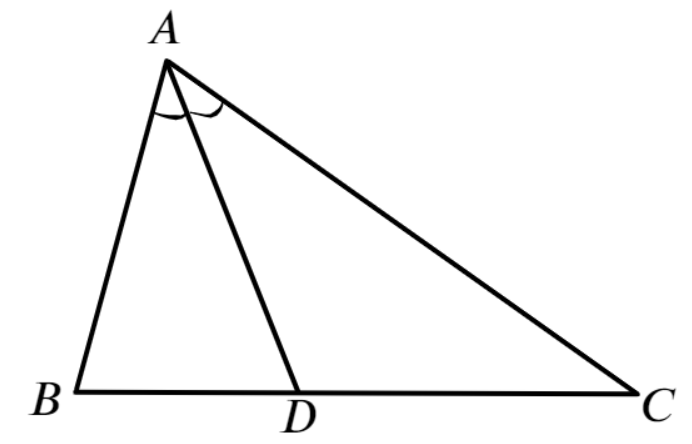
\includegraphics[scale=0.35]{g8-127.png}}
\end{figure}\\
По теореме об основании биссектрисы $\cfrac{BD}{DC}=\cfrac{AB}{AC}=\cfrac{3}{5}.$ У треугольников $ABD$ и $ACD$ общая высота, опущенная из точки $A,$ значит $\cfrac{S_{\Delta ABD}}{S_{\Delta ACD}}=\cfrac{BD}{DC}=\cfrac{3}{5},$ значит $S_{\Delta ACD}=S_{\Delta ABD}\cdot \cfrac{5}{3}=9\cdot\cfrac{5}{3}=15\text{ см}^2.$\\
